\documentclass{svproc}
\usepackage{graphicx} 
\usepackage{amsmath}
\usepackage{biblatex}
\addbibresource{lit.bib}

\title{Exploring the effectiveness of Small-Scale Vision and Language Models for Vision and Language Navigation Tasks in Continuous Environments}
\author{Wesley Chiu, Abdulrahman Altahhan}
\institute{University of Leeds, School of Computing, ODL MSc in AI, UK.}
\date{January 2025}

\begin{document}
\maketitle

\begin{abstract}
    Vision-and-Language Navigation (VLN) is a rapidly evolving field of research that aims to enable an embodied agent to follow textual instructions given in natural language to navigate through an unseen environment to a goal position. Existing approaches to this ask all into two main categories: "specialist" models that have been constructed and trained specifically to solve this task, and zero-shot or few-shot models that aim to leverage the implicit knowledge within Large Language Models (LLMs) and Vision Language Models  (VLMs). Prior work in the latter approach have used the most powerful models (70B+ parameters). This work aims to evaluate the suitability of using a lighter-weight variant of an existing open-sourced model (Qwen2-VL) as the primary VLM, which would allow it to be run "on-device" rather than being connected to a broader network. The experiments in a simulated environment demonstrates that the current ability of the lighter-weight model is not yet fit for purpose, failing to reach the success rates 
    seen approaches that use the full-sized variants.
    
    \keywords{Vision-and-Language Navigation, Vision Language Model, Large Language Model, Prompt Engineering, Prompting}
\end{abstract}

\section{Introduction}
    Vision-and-Language Navigation (VLN) is a rapidly evolving field of research, which tasks an embodied agent to follow a set of textual instructions given in natural language to navigate a previously unseen 3D indoor environment. Whilst initial research leveraged models such as RNNs and CNNs to process visual and natural language data, the introduction of Transformer-based models \cite{attenion_is_all_you_need} has accelerated capabilities in Natural Language Processing (NLP) and Computer Vision (CV) - both key components in the VLN task. The rapid development of Large Language Models (LLMs) and Vision-Language Models (VLMs) has further intensified the volume and pace of research in VLN, with each advance in LLM and VLM competency directly benefiting the VLN task.
    The traditional VLN task, as proposed by \cite{8578485}, has the agent navigating between pre-defined nodes in the environment (sometimes referred to as a navigation graph), which essentially reduces the VLN task to a vision-based graph-search problem; models trained in this manner have difficulty translating to performance in the real-world \cite{pmlr-v155-anderson21a}. To help combat this gap, the VLN Continuous Environment (VLN-CE) task was introduced, and has no such predefined navigation points, allowing agents to take any action to reach a navigable point in the environment; this introduces new challenges for the models to overcome, such as avoiding getting stuck on obstacles and dealing with distances \cite{krantz2020navgraphvisionandlanguagenavigationcontinuous}.
    \newline
    Approaches to the VLN task (whether traditional VLN or VLN-CE) that leverage existing LLMs and VLMs typically fall into two broad categories: zero-shot approaches or 'specialist' models.
    Zero-shot models \cite{long2023_discussnav, chen2024mapgptmapguidedpromptingadaptive, zhou2023navgptexplicitreasoningvisionandlanguage} aim to leverage the implicit knowledge, NLP ability, and strong reasoning skills within LLMs and VLMs \cite{CITATION_NEEDED} to navigate the environment. These models rely on specific prompting to generate historical trajectories, make navigation decisions, and to monitor progress. However, these models typically rely on translating visual data into purely textual information, which risks a loss of information in the process \cite{pan2024langnavlanguageperceptualrepresentation}; as a result, these models typically underperform against specialist models. The strength of these models lie in the fact that no pre-training is required, and as LLMs and VLMs continue to improve, this increase in competency can directly translate into improved VLN performance without the need for pre-training or adaptation of a complex model structure.
    \newline
    Specialist models \cite{hong2021_vlnbert, navgpt2, chen2021_HAMT, HE2024110511_MemoryAdaptiveVLN} are those that either take an off-the-shelf LLM or VLM and finetune the model for the VLN task, or are models (usually consisting of multiple sub-models) specifically finetuned and constructed to tackle the VLN task. These models exhibit much improved performance in VLN tasks, but cannot take advantage of more competent LLMs or VLMs as they are released.
    \newline
    Against this background, this work proposes to use a finetuned open-source model as its primary VLM, using QLoRA \cite{citatation_required} to finetune the very capable Qwen2-VL-7B variant \cite{citation_required}.
    
\section{Literature Review}
    \cite{TD0-Replay} has established a new TD(0) method that replays all past experiences. On the hand, \cite{TD-Replay} has taken this further to include a target that incorporates all past updates via TD($\lambda$). \cite{ConjugateTD} applied conjugate gradient update on TD.


\section{Methodology}
    In this section, we lay out the methodology. Note how in Fig. \ref{fig:my_label} we have shown the boundary.


    \begin{figure}
        \centering
        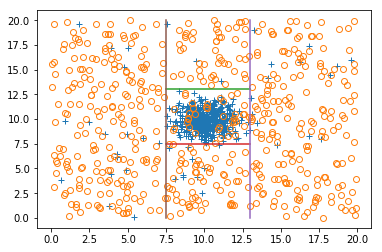
\includegraphics[scale=.75]{figures/DecisionBoundary.png}
        \caption{Caption}
        \label{fig:fig2}
    \end{figure}

    
    \begin{figure}
        \centering
        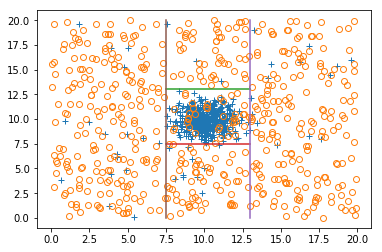
\includegraphics[scale=.75]{figures/DecisionBoundary.png}
        \caption{Caption}
        \label{fig:my_label}
    \end{figure}


    
    In Fig. \ref{fig:my_label} that $\alpha = n^2$. In eq. (\ref{eq:sum_i}) we have shown that the $ 1+2+3+4 = 4\times 5 /2=10$.
    \begin{align*}
        \sum_{i=1}^{n} y &= 10 \\
        M &= \beta ^2 \\
        \boldsymbol{B}^\top &= \boldsymbol{\Lambda}^2 \\
    \end{align*}
    
    \begin{align}
        \label{eq:sum_i}
        \sum_{i=1}^n i &= \frac{(n+1)n}{2} \\  
        \nonumber
        \beta ^2 &= \alpha_i^n
    \end{align}

\section{Experiment Results}
    \subsection{Experiment 1}
        \subsubsection{Exp}
    Note that the figure and the tables might be laid out on another page. Do not worry about that, and do not attempt to change it. Leave this to Latex.
    
    
    \begin{table}
        \caption{This is a table}
        \begin{center}
            \begin{tabular}{rlc}
                \hline
                \multicolumn{1}{l}{Year}&\multicolumn{1}{l}{World}&\multicolumn{1}{l}{Duration}\\
                \hline
                8000 B.C.  &     5,000,000 &  10\\
                  50 A.D.  &   200,000,000 &  20\\
                1650 A.D.  &   500,000,000 &  30\\
                \hline
            \end{tabular}
        \end{center}
    \end{table}

\section{Conclusion and Future Work}
We have conducted a study on ...

\printbibliography 
\end{document}
